\chapter{Concept Assessment}\label{cha:assessment}

- Survey
- Performance measures
- Limitations

\section{Levels}

    \subsection{Interaction}

        The scenario described is illustrated in Figure~\ref{fig:ui1}.

        \begin{figure}[htbp]
            \centering
            % \begin{tikzpicture}
            %     \draw[black, dashed, thin, fill=black!5] (0,0) rectangle (\linewidth,4);
            % \end{tikzpicture}
            \begin{lstlisting}[language=Bash]
Publisher initializing.
[INFO] [168766.57900] [wasm_cpp]: Context initializing.
[INFO] [168767.91500] [wasm_publisher]: Publishing: 'Hello there! 0'
[INFO] [168768.98400] [wasm_publisher]: Publishing: 'Hello there! 1'
[INFO] [168769.94400] [wasm_publisher]: Publishing: 'Hello there! 2'
[INFO] [168770.90300] [wasm_publisher]: Publishing: 'Hello there! 3'
[INFO] [168771.96800] [wasm_publisher]: Publishing: 'Hello there! 4'
[INFO] [168772.92000] [wasm_publisher]: Publishing: 'Hello there! 5'
[INFO] [168773.97600] [wasm_publisher]: Publishing: 'Hello there! 6'
[INFO] [168774.93600] [wasm_publisher]: Publishing: 'Hello there! 7'
\end{lstlisting}
            \caption{Output from non-interactive Level 1.}\label{fig:ui1}
        \end{figure}

        \begin{tcolorbox}[title=Example 1]
            \begin{minipage}[t]{0.87\linewidth}
                \vspace*{0pt}
                A demonstration of a \textit{non-interactive} user interface (Level 1) can
                be found at \href{https://ros2wasm.dev/pages/demo01/index.html}{\textsf{ros2wasm.dev/pages/demo01}}

                \textsc{Note:} The page must be reloaded to restart the node.
            \end{minipage}\hfill%
            \begin{minipage}[t]{0.1\linewidth}
                \vspace*{0pt}
                
\includegraphics[height=\linewidth,width=\linewidth]{qr_demo01.png}
            \end{minipage}
        \end{tcolorbox}


        Level 2 is exhibited in Figure~\ref{fig:ui2}

        \begin{figure}[htbp]
            \centering
            % 
\includegraphics[width=\linewidth]{03_level2.png}
            \begin{tikzpicture}
                \node (start) [
                    box,
                    xshift = -5cm,
                    minimum width = 2.5cm,
                ] {\footnotesize{\textbf{START}}};
                \node (stop) [
                    box,
                    minimum width = 2.5cm,
                    fill = igmrLightBlue,
                ] {\footnotesize{\textbf{STOP}}};
                \node (clear) [
                    box,
                    xshift = 5cm,
                    minimum width = 2.5cm,
                ] {\footnotesize{\textbf{CLEAR}}};
            \end{tikzpicture}
            \begin{lstlisting}[language=Bash]
[INFO] [16879468.55200] [wasm_publisher]: Publishing: 'Hello there! 13'
[INFO] [16879469.60800] [wasm_publisher]: Publishing: 'Hello there! 14'
[INFO] [16879470.56000] [wasm_publisher]: Publishing: 'Hello there! 15'
[INFO] [16879471.61600] [wasm_publisher]: Publishing: 'Hello there! 16'
[INFO] [16879472.56800] [wasm_publisher]: Publishing: 'Hello there! 17'
[INFO] [16879473.62400] [wasm_publisher]: Publishing: 'Hello there! 18'
Publisher terminated.\end{lstlisting}
            \caption{Interactive buttons to start and stop the publisher node.}\label{fig:ui2}
        \end{figure}

        \begin{tcolorbox}[title=Example 2]
            \begin{minipage}[t]{0.87\linewidth}
                \vspace*{0.5\baselineskip}
                A demonstration of a \textit{minimal} user interface (Level 2) can
                be found at \href{https://ros2wasm.dev/pages/demo02/index.html}{\textsf{ros2wasm.dev/pages/demo02}}
            \end{minipage}\hfill%
            \begin{minipage}[t]{0.1\linewidth}
                \vspace*{0pt}
                
\includegraphics[height=\linewidth,width=\linewidth]{qr_demo02.png}
            \end{minipage}
        \end{tcolorbox}

        Figure~\ref{fig:ui3} demonstrates a snapshot of Level 3.

        \begin{figure}[htbp]
            \centering
            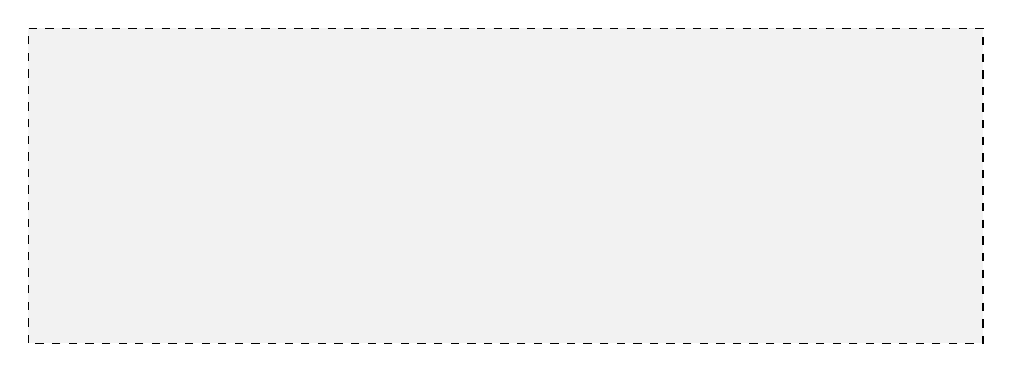
\begin{tikzpicture}
                \draw[black, dashed, thin, fill=black!5] (0,0) rectangle (\linewidth,4);
                \end{tikzpicture}
            \caption{TODO Level 3 image}\label{fig:ui3}
        \end{figure}

        \begin{tcolorbox}[title=Example 3]
            \begin{minipage}[t]{0.87\linewidth}
                \vspace*{0.5\baselineskip}
                A demonstration of a \textit{basic} user interface (Level 3) can
                be found at \href{https://ros2wasm.dev/pages/demo03/index.html}{\textsf{ros2wasm.dev/pages/demo03}}
            \end{minipage}\hfill%
            \begin{minipage}[t]{0.1\linewidth}
                \vspace*{0pt}
                
\includegraphics[height=\linewidth,width=\linewidth]{qr_demo03.png}
            \end{minipage}
        \end{tcolorbox}

        A depiction of Level 4 is shown in Figure~\ref{fig:ui4}

        \begin{figure}[htbp]
            \centering
            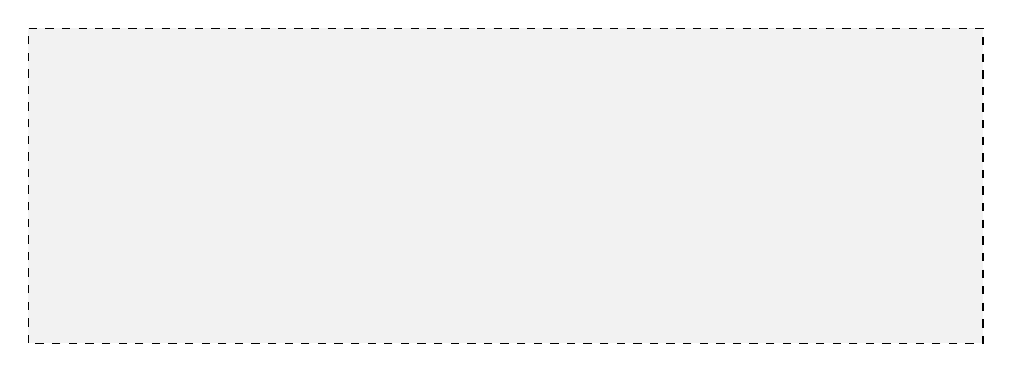
\begin{tikzpicture}
                \draw[black, dashed, thin, fill=black!5] (0,0) rectangle (\linewidth,4);
                \end{tikzpicture}
            \caption{TODO Level 4 image}\label{fig:ui4}
        \end{figure}

        \begin{tcolorbox}[title=Example 4]
            \begin{minipage}[t]{0.87\linewidth}
                \vspace*{0.5\baselineskip}
                A demonstration of an \textit{intermediate} user interface (Level 4) can
                be found at \href{https://ros2wasm.dev/pages/demo04/index.html}{\textsf{ros2wasm.dev/pages/demo04}}
            \end{minipage}\hfill%
            \begin{minipage}[t]{0.1\linewidth}
                \vspace*{0pt}
                
\includegraphics[height=\linewidth,width=\linewidth]{qr_demo04.png}
            \end{minipage}
        \end{tcolorbox}

        A typical workspace in JupyterLite is pictured in Figure~\ref{fig:ui5}.

        \begin{figure}[htbp]
            \centering
            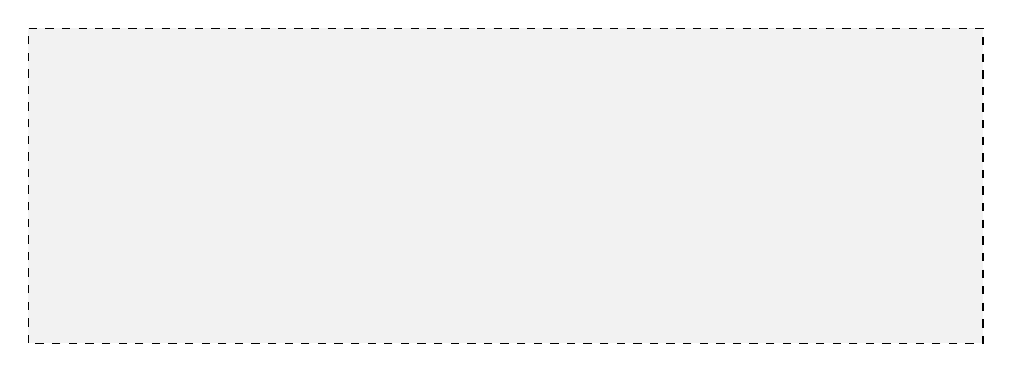
\begin{tikzpicture}
                \draw[black, dashed, thin, fill=black!5] (0,0) rectangle (\linewidth,4);
                \end{tikzpicture}
            \caption{TODO Level 5 image}\label{fig:ui5}
        \end{figure}

        % NO DEMO HERE
        % \begin{tcolorbox}[title=Example 5]
        %     \begin{minipage}[t]{0.87\linewidth}
        %         \vspace*{0.5\baselineskip}
        %         A demonstration of an \textit{advanced} user interface (Level 5) can
        %         be found at \href{https://ros2wasm.dev/pages/demo05/index.html}{\textsf{ros2wasm.dev/pages/demo05}}
        %     \end{minipage}\hfill%
        %     \begin{minipage}[t]{0.1\linewidth}
        %         \vspace*{0pt}
        %         
\includegraphics[height=\linewidth,width=\linewidth]{qr_demo05.png}
        %     \end{minipage}
        % \end{tcolorbox}
